\documentclass[../main.tex]{subfiles}
\begin{document}

\subsection{QCD multi-jet}
\label{hh:subs:qcd}


Generic QCD multi-jet events can enter the final selection if two jets are misidentified as the $\tau\tau$ pair. The process creating QCD multi-jets has the largest cross section among all the background processes so, event it gets reduced thanks to the analysis selections, its contribution ends up being notably important, particularly in the $\tau_h\tau_h$ channel. Estimating the QCD background contribution via simulated events would require a prohibitively large number of them, so the estimation is performed using a data-driven method. The strategy used is often called ``ABCD'' method, and is described as follows.


\subsubsection{QCD background estimation using the ABCD method}

The ABCD takes its name from the fact that 4 regions are used: the signal region, A, and three other regions, B, C and D, obtained by reverting two different selection criteria. In the HH$\to$bb$\tau\tau$ analysis, region B (\textit{same-sign, isolated}) is obtained by inverting the tau pair charge requirement. In region C (\textit{opposite-sign, non-isolated}), the DeepTauVsJet selection is inverted by requiring that the selected $\tau_h$ (the one with the lowest $p_t$ in the $\tau_h\tau_h$ channel) fails the medium working point but still passes the VVVLoose one. Region D (\textit{same-sign, non-isolated}) combines these two inverted selections. An sketch of the four regions is shown in Fig.~\ref{hh:fig:qcd_sketch}.

\begin{figure}[h!]
\begin{center}
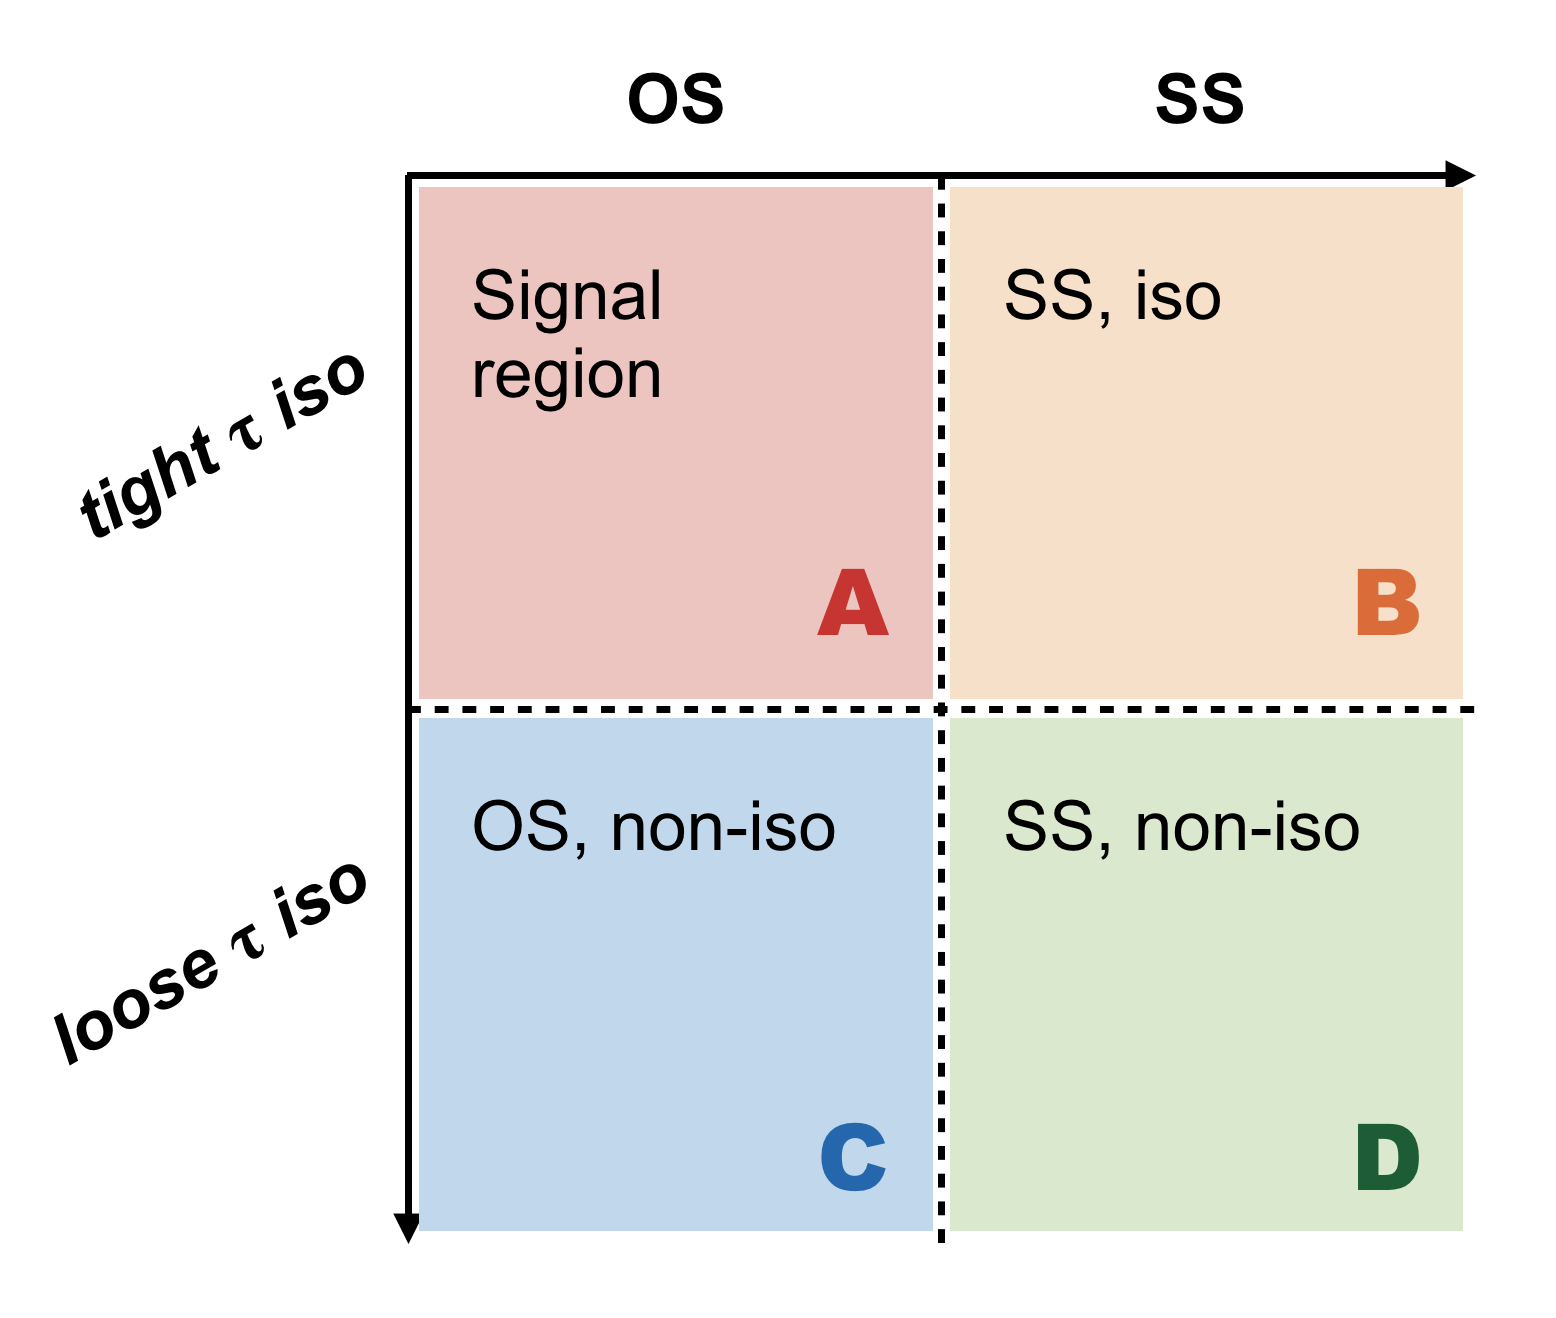
\includegraphics[width=0.5\textwidth]{Images/QCDschema}
\end{center}
\caption{Sketch of the four regions used to estimate the QCD multi-jet background.}
\label{hh:fig:qcd_sketch}
\end{figure}

The distribution of the multi-jet QCD contribution in any given binned variable is estimated from the C region: yields from the other backgrounds are substracted from the data in this region and the remaining number of events in each bin is then multiplied by a factor $k^{\text{iso/non-iso}}$. This factor tries to account for moving from the non-isolated selection (present in region C) to the isolated selection (used in the signal region), and is measured as the ratio of event yields in regions B and after substracting the other background yields in each region. Therefore, the ABCD method gives a QCD estimation whose shape comes from the data - background shape in region C and its yield from the data - background yields from regions B, C and D as given by the formula C $\times$ B / D. However, in some analysis categories due to the lack of statistics, a different selection is applied to regions B and D. In the boosted category, the B / D ratio is computed with all the selections defined in the category excluding the b-tagging requirement, while in the five VBF subcategories, the B / D correction factor is estimated from the VBF inclusive category, which includes the five subcategories.



\subsubsection{Validity tests for the QCD background estimation}

In order to evaluate the validity of the followed procedure, several tests were performed. Details and results of these tests are given here.

In the first test, the stability of the estimated QCD normalization has been evaluated by modifying the definition of the C and D regions using four different \deeptau{} working points. These alternative regions are defined as:
\begin{itemize}
\item Events where the \tauh{} passes the VVVLoose working point of the DeepTauVSjet discriminator, but not the VVLoose one.
\item Events where the \tauh{} passes the VVLoose working point of the DeepTauVSjet discriminator, but not the VLoose one.
\item Events where the \tauh{} passes the VLoose working point of the DeepTauVSjet discriminator, but not the Loose one.
\item Events where the \tauh{} passes the Loose working point of the DeepTauVSjet discriminator, but not the Medium one.
\end{itemize}

In these four alternative regions the ratio between the C and D yields is computed and compared with the one obtained with the standard definition of the C and D regions. Results for the C/D yield estimation for the \tauh\tauh{} channel (where the QCD contribution is really important) in 2018 are shown in Fig.~\ref{hh:fig:qcd_test1} \textcolor{red}{(Other channels and years here or in appendix?)}. A straight line showing a fit to a constant of the C/D yield values for the four alternative working point definitions is also plotted. When a working point leads to a negative yield in either of regions B, C or D, a dashed band is shown and the point is not used to compute the fit nor the average. In general the C/D yield obtained with the standard definition of C and D regions is in agreement within uncertainties with both the result of this constant fit, and with the weighted average of these four alternative C/D yield points. In the few cases where this does not happen, an additional uncertainty is proposed, as defined in Section~\ref{hh:sec:systematics}.

\begin{figure}[h!]
\begin{center}
\subfloat[Boosted]{\includegraphics[width=0.3\textwidth]{Images/qcd_tests/2018/boosted/qcd_inviso__tautau.pdf}}
\subfloat[Resolved, 1 b-tag]{\includegraphics[width=0.3\textwidth]{Images/qcd_tests/2018/resolved_1b/qcd_inviso__tautau.pdf}}
\subfloat[Resolved, 2 b-tag]{\includegraphics[width=0.3\textwidth]{Images/qcd_tests/2018/resolved_2b/qcd_inviso__tautau.pdf}}\\
\subfloat[VBF subcategory]{\includegraphics[width=0.3\textwidth]{Images/qcd_tests/2018/vbf/hh_vbf_sm_c2v/qcd_inviso__tautau.pdf}}
\subfloat[ggF subcategory]{\includegraphics[width=0.3\textwidth]{Images/qcd_tests/2018/vbf/hh_ggf/qcd_inviso__tautau.pdf}}
\subfloat[$\text{t}\bar{\text{t}}$ subcategory]{\includegraphics[width=0.3\textwidth]{Images/qcd_tests/2018/vbf/tt/qcd_inviso__tautau.pdf}}\\
\subfloat[$\text{t}\bar{\text{t}}$H subcategory]{\includegraphics[width=0.3\textwidth]{Images/qcd_tests/2018/vbf/ttH/qcd_inviso__tautau.pdf}}
\subfloat[DY subcategory]{\includegraphics[width=0.3\textwidth]{Images/qcd_tests//2018/vbf/dy/qcd_inviso__tautau.pdf}}\\
\end{center}
\caption{C/D yield estimations for the five working points for the \tauh\tauh{} channel in 2018. A dashed band is plotted where the correspondent working point leads to a negative yield for regions B, C and/or D.}
\label{hh:fig:qcd_test1}
\end{figure}

In the second test, the QCD estimation obtained from the ABCD method is compared with a direct data - background substraction in a sideband region where signal presence is negligible. This sideband region has been defined by inverting the elliptic mass cut (defined in Section~\ref{hh:sec:event_categorization} from the Resolved 1 b-tag category. Fig~\ref{hh:fig:qcd_test2_dnn} shows the DNN output distribution per channel and year in the sideband region considered. Again the QCD estimation obtained with ABCD method has been found to be in good agreement with the direct data-background subtraction in this sideband, validating the QCD estimations obtained with the ABCD method used in the analysis.

\begin{figure}
\centering
\subfloat[$\tau_e\tau_h$, 2016]{\includegraphics[width=0.33\textwidth]{Images/qcd_tests/2016/resolved_1b_inv/DNNoutSM_kl_1__pg_plots__qcd__etau_os_iso__stack}}
\subfloat[$\tau_\mu\tau_h$, 2016]{\includegraphics[width=0.33\textwidth]{Images/qcd_tests/2016/resolved_1b_inv/DNNoutSM_kl_1__pg_plots__qcd__mutau_os_iso__stack}}
\subfloat[$\tau_h\tau_h$, 2016]{\includegraphics[width=0.33\textwidth]{Images/qcd_tests/2016/resolved_1b_inv/DNNoutSM_kl_1__pg_plots__qcd__tautau_os_iso__stack}}\\
\subfloat[$\tau_e\tau_h$, 2017]{\includegraphics[width=0.33\textwidth]{Images/qcd_tests/2017/resolved_1b_inv/DNNoutSM_kl_1__pg_plots__qcd__etau_os_iso__stack}}
\subfloat[$\tau_\mu\tau_h$, 2017]{\includegraphics[width=0.33\textwidth]{Images/qcd_tests/2017/resolved_1b_inv/DNNoutSM_kl_1__pg_plots__qcd__mutau_os_iso__stack}}
\subfloat[$\tau_h\tau_h$, 2017]{\includegraphics[width=0.33\textwidth]{Images/qcd_tests/2017/resolved_1b_inv/DNNoutSM_kl_1__pg_plots__qcd__tautau_os_iso__stack}}\\
\subfloat[$\tau_e\tau_h$, 2018]{\includegraphics[width=0.33\textwidth]{Images/qcd_tests/2018/resolved_1b_inv/DNNoutSM_kl_1__pg_plots__qcd__etau_os_iso__stack}}
\subfloat[$\tau_\mu\tau_h$, 2018]{\includegraphics[width=0.33\textwidth]{Images/qcd_tests/2018/resolved_1b_inv/DNNoutSM_kl_1__pg_plots__qcd__mutau_os_iso__stack}}
\subfloat[$\tau_h\tau_h$, 2018]{\includegraphics[width=0.33\textwidth]{Images/qcd_tests/2018/resolved_1b_inv/DNNoutSM_kl_1__pg_plots__qcd__tautau_os_iso__stack}}
    \caption{DNN output distribution per channel for the sideband region defined by inverting the elliptic mass cut in the Resolved 1 b-tag category.  Statistical uncertainties for the data and all background contributions and the normalization systematic uncertainties for the main background processes are included.}
    \label{hh:fig:qcd_test2_dnn}
\end{figure}

Finally, the last validity test consists of obtaining the QCD contribution using the ABCD method in the final analysis categories but redefining the usual regions using an alternative DeepTauVSjet working point that was already introduced in the first test. This way, the new regions A', B', C' and D' use the following selections:
\begin{itemize}
	\item A': Both $\tau$ have opposite charge and the $\tau_h$ passes the VVLoose working point but not the VLoose one.
	\item B': Both $\tau$ have the same charge and the $\tau_h$ passes the VVLoose working point but not the VLoose one.
	\item C': Both $\tau$ have opposite charge and the $\tau_h$ passes the VVVLoose working point but not the VVLoose one.
	\item C': Both $\tau$ have the same charge and the $\tau_h$ passes the VVVLoose working point but not the VVLoose one.
\end{itemize}

This way, we can estimate the QCD contribution in regions close to the analysis signal regions but poorly populated in signal (thanks to considering a very loose working point) and enhanced in QCD contribution. Fig.~\ref{hh:fig:qcd_test3_dnn} shows the DNN output distributions for the \tauh\tauh{} channel in 2018 in this alternative signal region. Agreement within the statistical uncertainties can be seen between the prediction from all background sources, including the QCD estimation obtained with the ABCD method, and the data in this validation region, reassuring the validity of the ABCD method for QCD estimation. In particular, we see a very big QCD contribution in the \tauh\tauh{} channel in the Resolved 1 b-tag category, where also a very good agreement within uncertainties between data and backgrounds can be observed.


\begin{figure}[h!]
\centering
\subfloat[Resolved, 1 b-tag]{\includegraphics[width=0.33\textwidth]{Images/qcd_tests/test3/2018/resolved_1b/DNNoutSM_kl_1__qcd__tautau_os_inviso__vvl_vl__stack__qcd_wp_vvvl_vvl.pdf}}
\subfloat[Resolved, 2 b-tag]{\includegraphics[width=0.33\textwidth]{Images/qcd_tests/test3/2018/resolved_2b/DNNoutSM_kl_1__qcd__tautau_os_inviso__vvl_vl__stack__qcd_wp_vvvl_vvl.pdf}}
\subfloat[Boosted ]{\includegraphics[width=0.33\textwidth]{Images/qcd_tests/test3/2018/boosted/DNNoutSM_kl_1__qcd__tautau_os_inviso__vvl_vl__stack__qcd_wp_vvvl_vvl.pdf}}\\
\subfloat[VBF subcategory]{\includegraphics[width=0.33\textwidth]{Images/qcd_tests/test3/2018/hh_vbf_sm_c2v/DNNoutSM_kl_1_hh_vbf_sm_c2v_merged_mpp__qcd__tautau_os_inviso__vvl_vl__stack__qcd_wp_vvvl_vvl.pdf}}
\subfloat[ggF subcategory]{\includegraphics[width=0.33\textwidth]{Images/qcd_tests/test3/2018/hh_ggf/DNNoutSM_kl_1_hh_ggf_merged_mpp__qcd__tautau_os_inviso__vvl_vl__stack__qcd_wp_vvvl_vvl.pdf}}
\subfloat[$\text{t}\bar{\text{t}}$ subcategory]{\includegraphics[width=0.33\textwidth]{Images/qcd_tests/test3/2018/tt/DNNoutSM_kl_1_tt_merged_mpp__qcd__tautau_os_inviso__vvl_vl__stack__qcd_wp_vvvl_vvl.pdf}}\\
\subfloat[$\text{t}\bar{\text{t}}$H subcategory]{\includegraphics[width=0.33\textwidth]{Images/qcd_tests/test3/2018/tth/DNNoutSM_kl_1_tth_merged_mpp__qcd__tautau_os_inviso__vvl_vl__stack__qcd_wp_vvvl_vvl.pdf}}
\subfloat[DY subcategory ]{\includegraphics[width=0.33\textwidth]{Images/qcd_tests/test3/2018/dy/DNNoutSM_kl_1_dy_merged_mpp__qcd__tautau_os_inviso__vvl_vl__stack__qcd_wp_vvvl_vvl.pdf}}
\caption{DNN output distribution for the different analysis categories in the alternative signal region defined by a looser DeepTauVSjet working point for the \tauh\tauh{} channel in 2018. Statistical uncertainties for the data and all background contributions are included.}
\label{hh:fig:qcd_test3_dnn}
\end{figure}




%\bibliographystyle{unsrt}
%\bibliography{../biblio.bib}



\end{document}

